\section{Results}

The procedure followed was to train the agents in different conditions and then test 
its performance across a variety of conditions, that is various initial states. 
Table~\ref{tab:benchmark_strategy} shows exactly what cases were contemplated. Testing conditions are elaborated on in the following section.

\begin{table}[H]
    \centering
    \caption{Benchmark strategy to compare different training settings and 
    initial testing conditions.}
    \label{tab:benchmark_strategy}
    \begin{tabular}{l | c c c}
        \toprule[0.5pt]
                                    & \multicolumn{3}{c}{\textbf{Initial testing condition}}    \\
        \textbf{Training condition}   & Vanilla     & Moderate      & Extreme                   \\
        \midrule[1pt]
        Vanilla                       & X           &  -            & -                         \\
        Moderate                      & X           &  X            & X                         \\
        Extreme                       & -           &  -            & X                         \\
        \bottomrule[2pt]
    \end{tabular}
\end{table}

\subsection{Training stage}

We trained the drone to hover in place (vanilla), to navigate to a goal point from a randomized starting state (moderate), and the same navigation tasks but harder initial conditions (extreme). These problem settings can be summarized in 
Table~\ref{tab:train_conditions}. 

The training was carried out through SpinningUp's interface, where we trained until the average return per epsiode leveled off. Each epoch in training consists of 6000 steps, and each epsiode has a maximum of 2000 steps. This means that epochs contain less episodes as the agent becomes better at the task. All hyperparameters were taken from the relevant algorithm's papers.

\begin{table}[H]
    \centering
    \caption{Training conditions.}
    \label{tab:train_conditions}
    \begin{tabular}{l|c p{25mm}}
        \toprule[0.5pt]
                                    & \multicolumn{2}{c}{\textbf{Configuration}}    \\
        \textbf{Training condition} & Random start & Initial State \\
        \midrule[1pt]
        Vanilla                     & No    &  null       \\
        \toprule[0.5pt]
        Moderate                    & Yes   &  $er_i < 1.2$ \newline 
                                               $|v_i| < 0.5$ \newline
                                               $|\phi|,|\theta|,|\psi|<\sfrac{\pi}{3}$ \newline
                                               $|\omega_i| < \sfrac{\pi}{10}$ \\
        \toprule[0.5pt]
        Extreme                     & Yes   &  $er_i < 1.2$ \newline 
                                               $|v_i| < 2.0$ \newline
                                               $|\phi|,|\theta|,|\psi|<\sfrac{\pi}{2}$ \newline
                                               $|\omega_i| < \sfrac{\pi}{3}$ \\
        \bottomrule[2pt]
    \end{tabular}
\end{table}

In addition to the strategy previously exposed, the training process was carried out by 
executing 5 runs of approximately\footnote{Some algorithms required less training} 50 epochs,
where an epoch represents 1000 episodes or 5000 steps.

The first algorithms used to tackle the problem were VPG, DDPG and PPO. However, the cumulative 
reward was nowhere near what was expected. The aforementioned can be appreciated in 
Figure~\ref{fig:failed_training}. As to why our training failed here, we are still a bit confused. Aside from what is shown here, we tried training VPG and PPO for a much longer time, and they still did not perform up to par.

\begin{figure}[H]
    \centering
     \begin{subfigure}[b]{\textwidth}
         \centering
             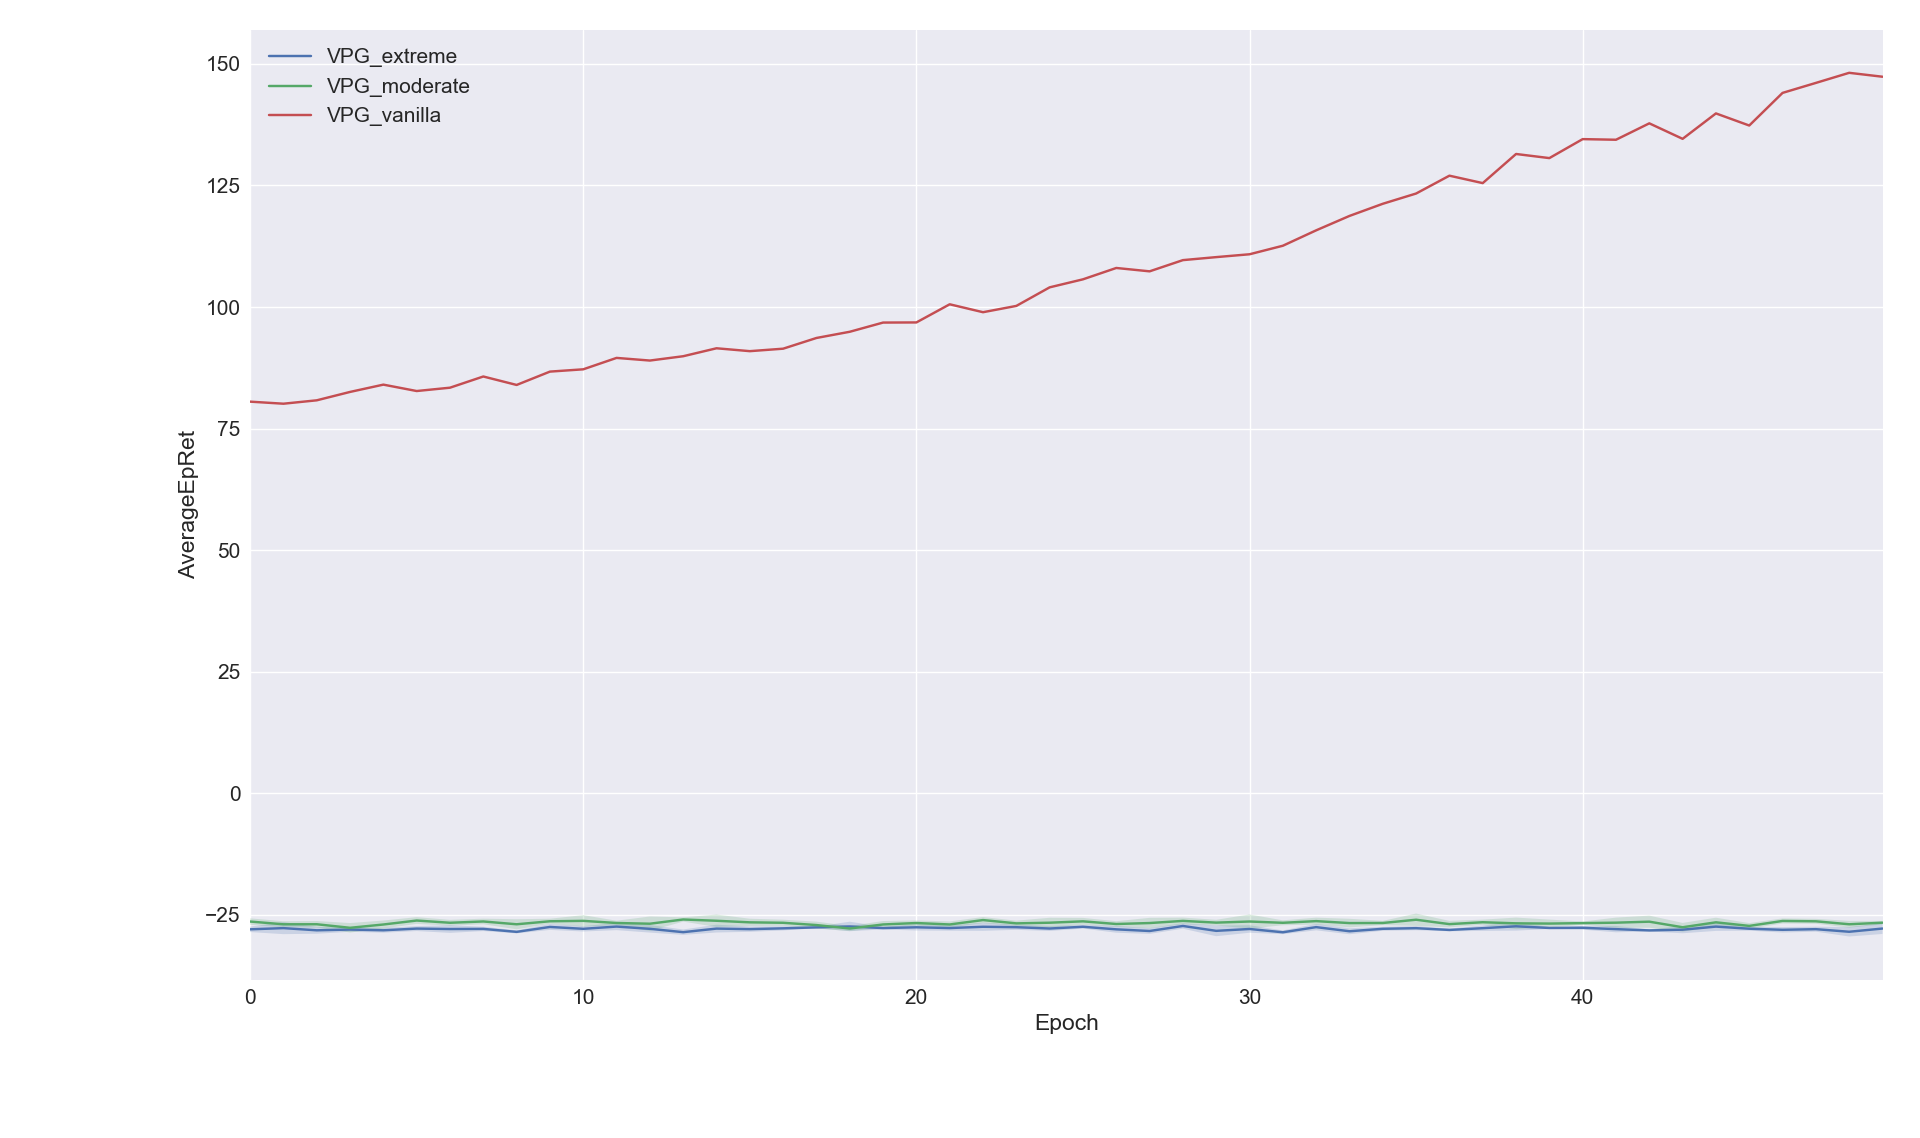
\includegraphics[width = 0.7\textwidth]{return_VPG.png}
     \end{subfigure}
    \vfill 
     \begin{subfigure}[b]{\textwidth}
         \centering
             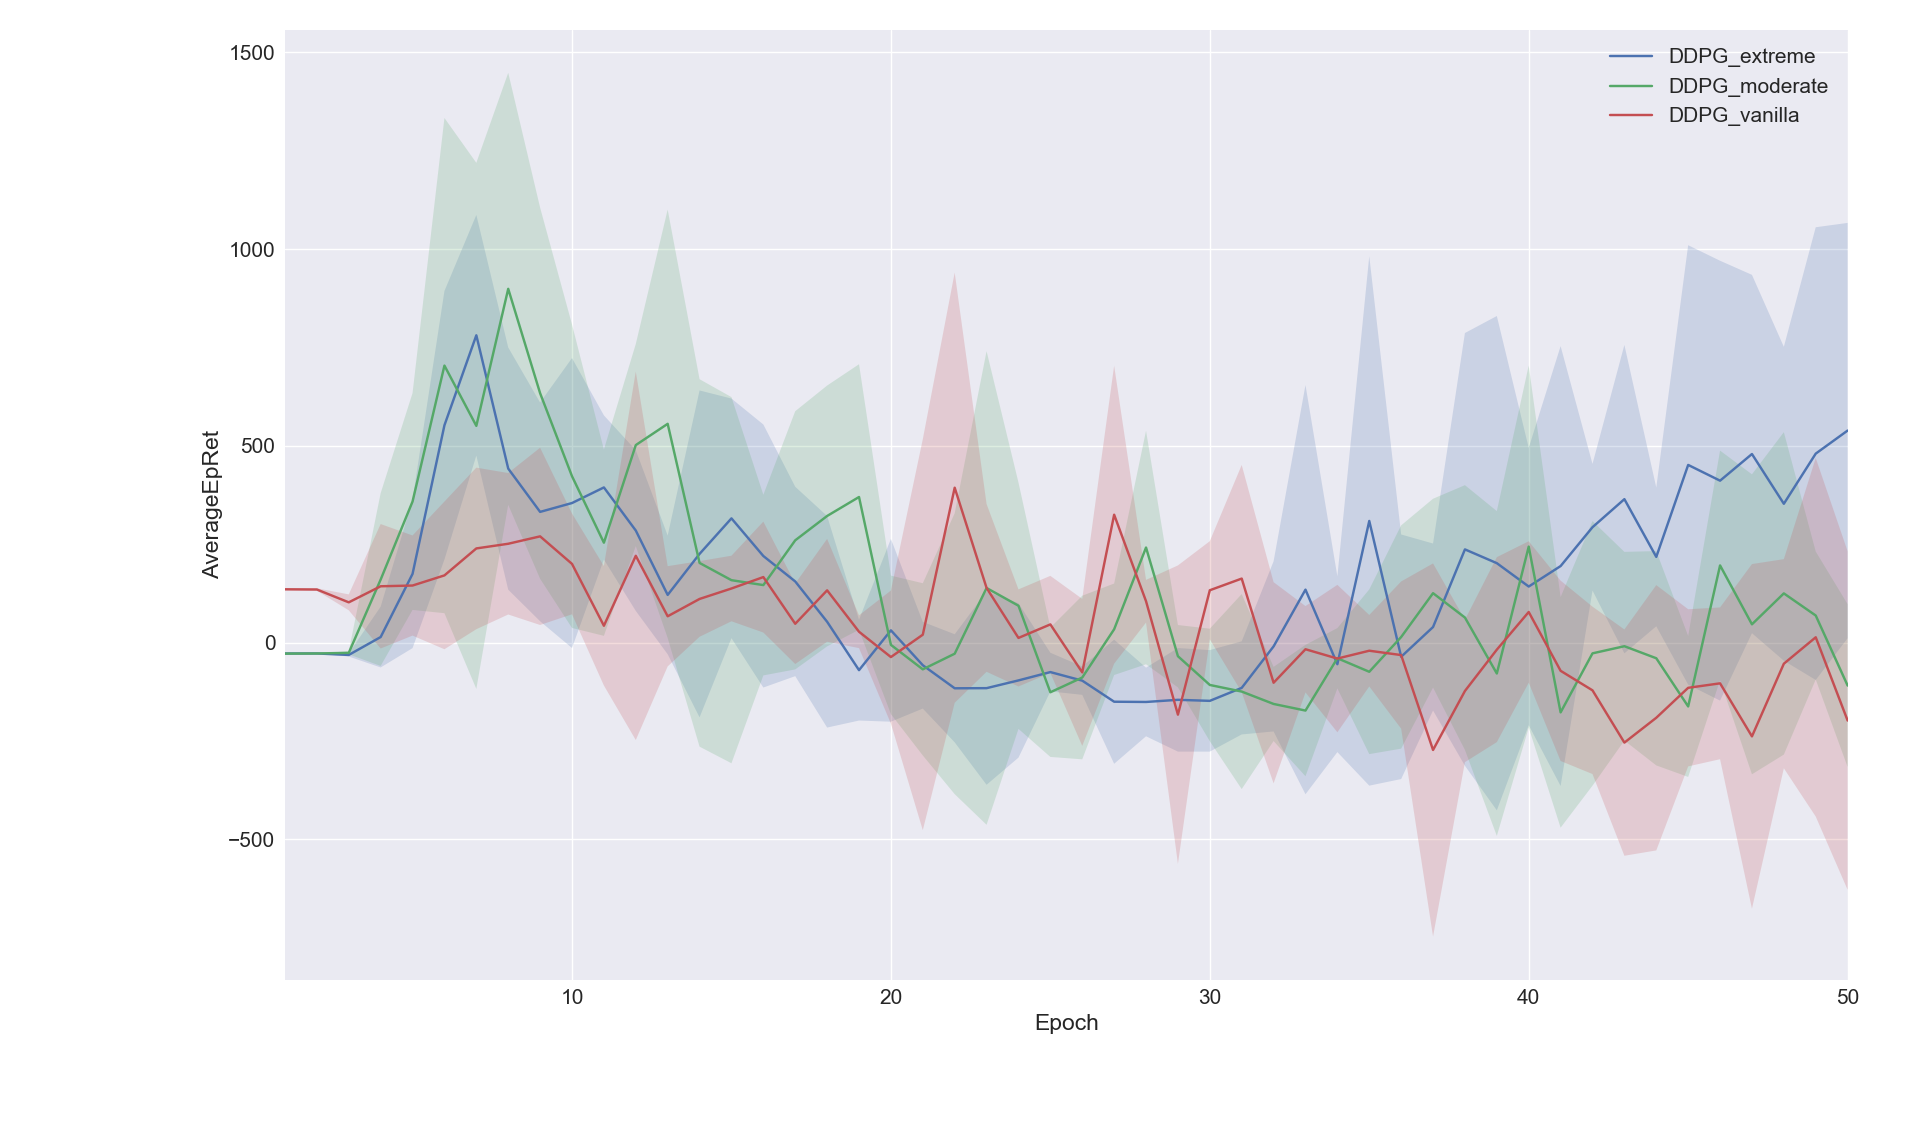
\includegraphics[width = 0.7\textwidth]{return_DDPG.png}
     \end{subfigure}
     \vfill
     \begin{subfigure}[b]{\textwidth}
         \centering
             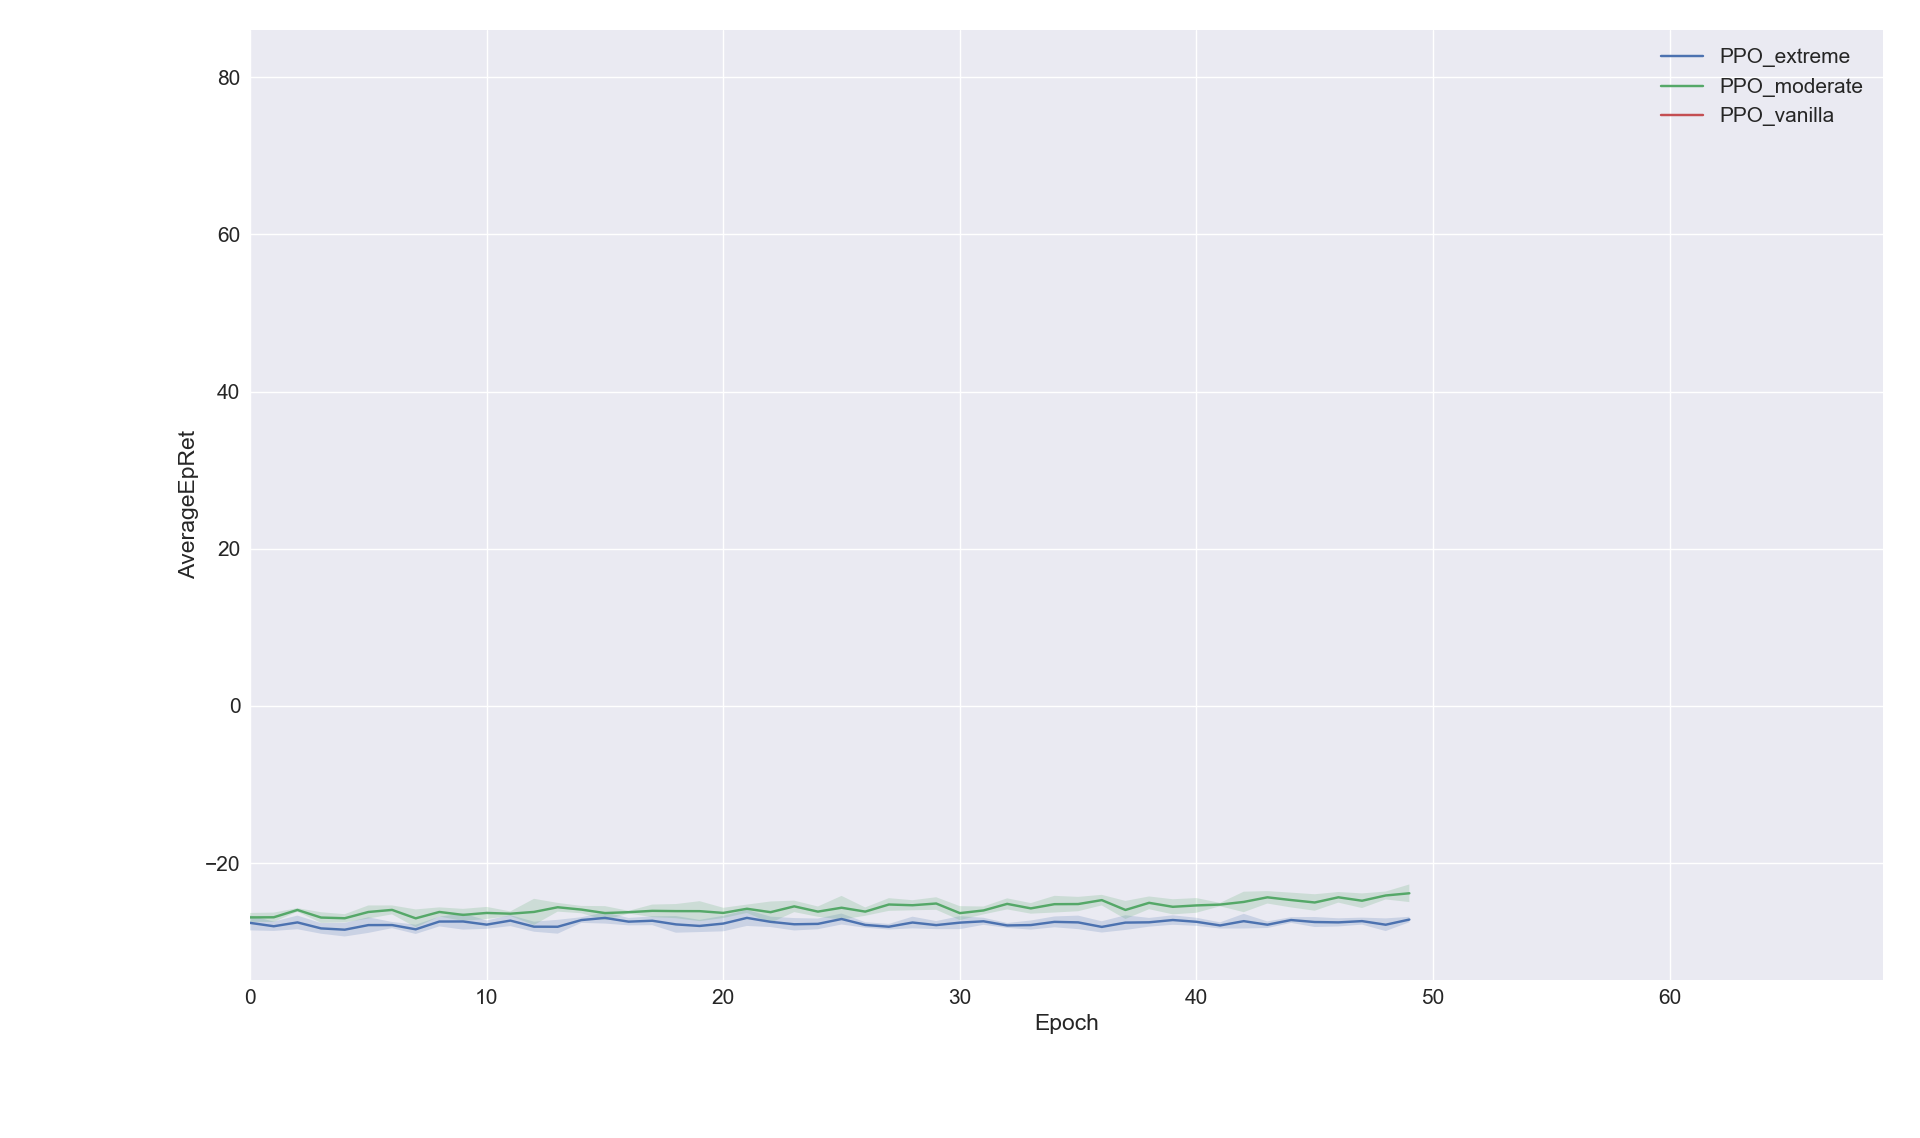
\includegraphics[width = 0.7\textwidth]{return_PPO.png}
     \end{subfigure}
    \caption{VPG, DDPG and PPO cumulative return for the vanilla training case. Given 
    that 5 runs were executed, the plot reflects the average and standard deviation 
    corresponding to the learning process of the 5 agents.}
    \label{fig:failed_training}
\end{figure}

We also trained on TD3 and SAC. In this case, the situation changed dramatically.
Within the first 20 epochs both algorithms were performing quite well, with more consistent results for TD3. Perhaps TD3 is more robust than SAC during training because it is trying to learn a deterministic policy rather than a stochastic policy, and entropy regularization encourages too much exploration. Figure~\ref{fig:sac} and Figure~\ref{fig:td3} reveal this. 

% \begin{figure}[H]
%     \centering
%      \begin{subfigure}[b]{\textwidth}
%          \centering
%              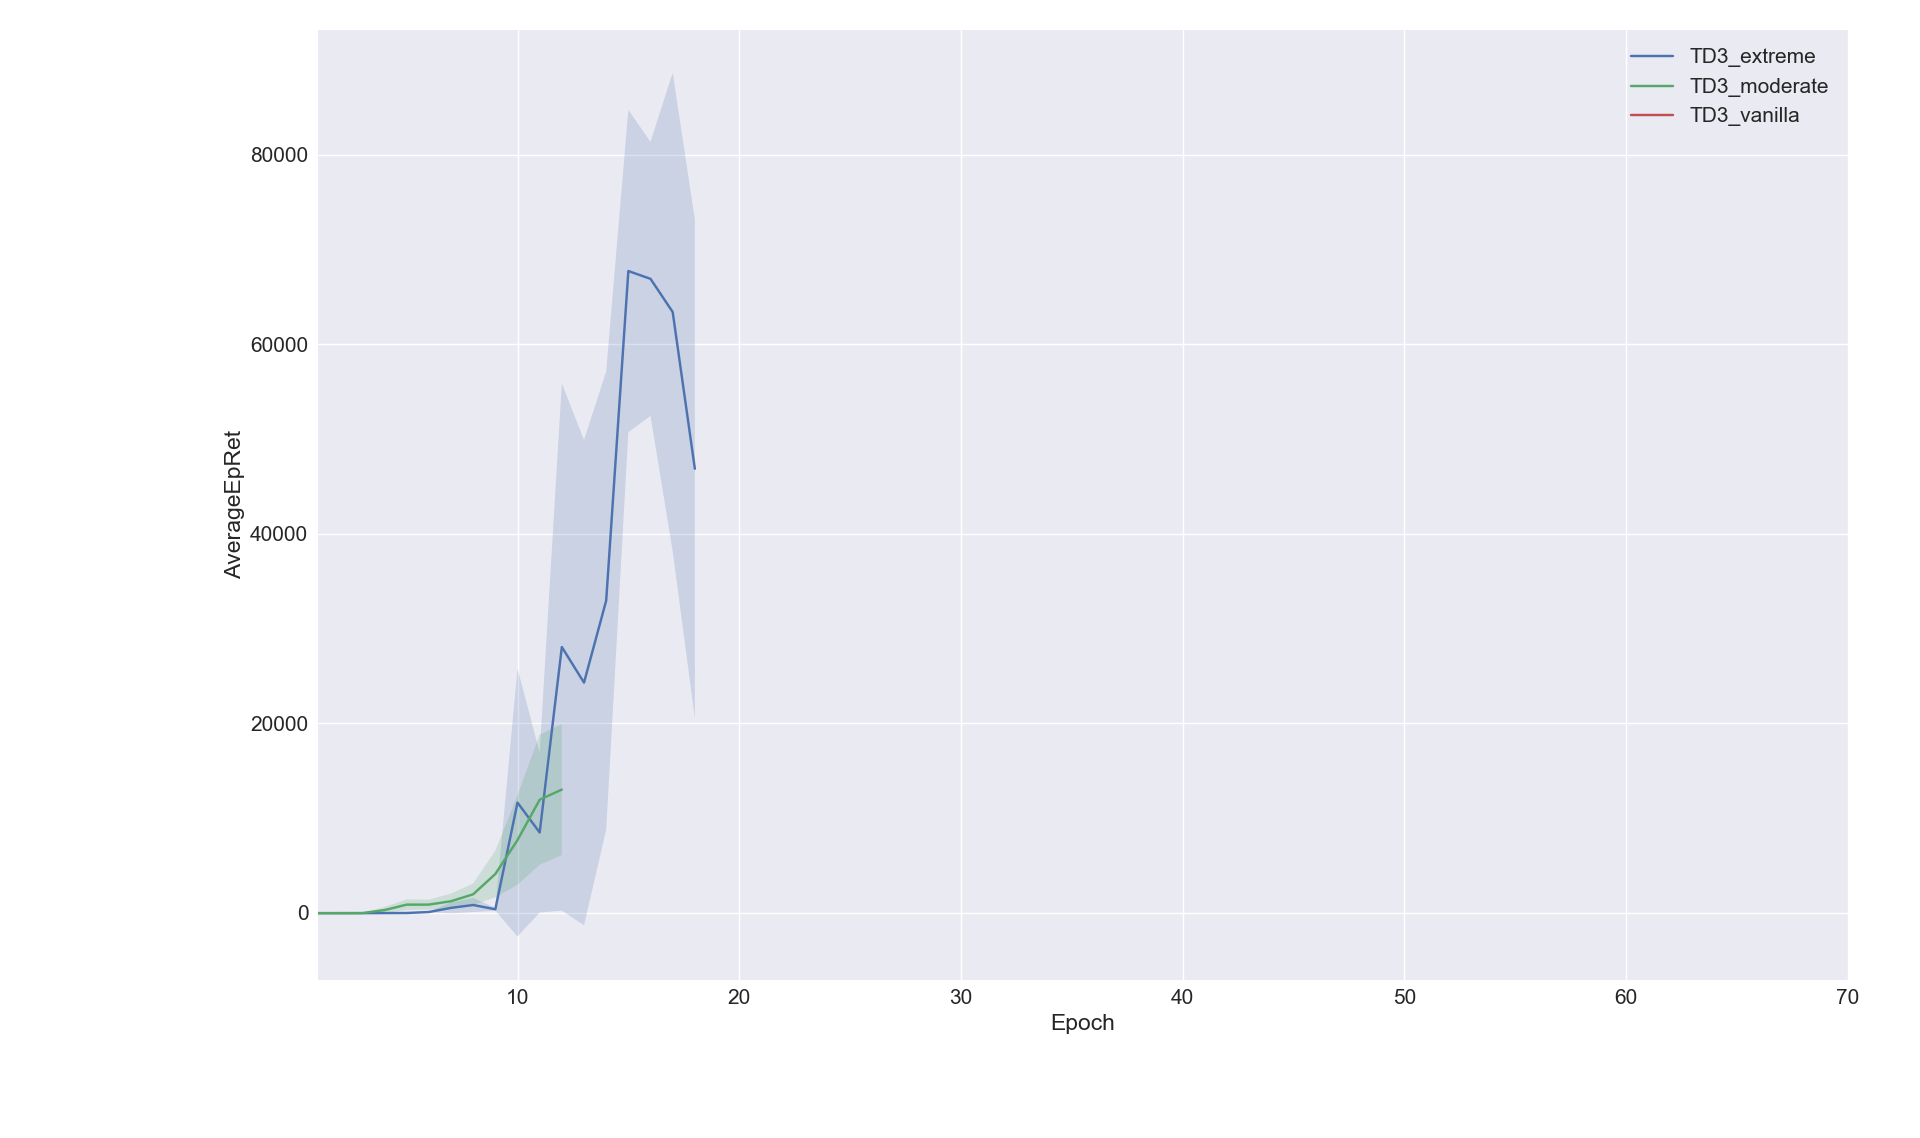
\includegraphics[width = .82\textwidth]{img/return_TD3.png}
%      \end{subfigure}
%      \vfill
%      \begin{subfigure}[b]{\textwidth}
%          \centering
%              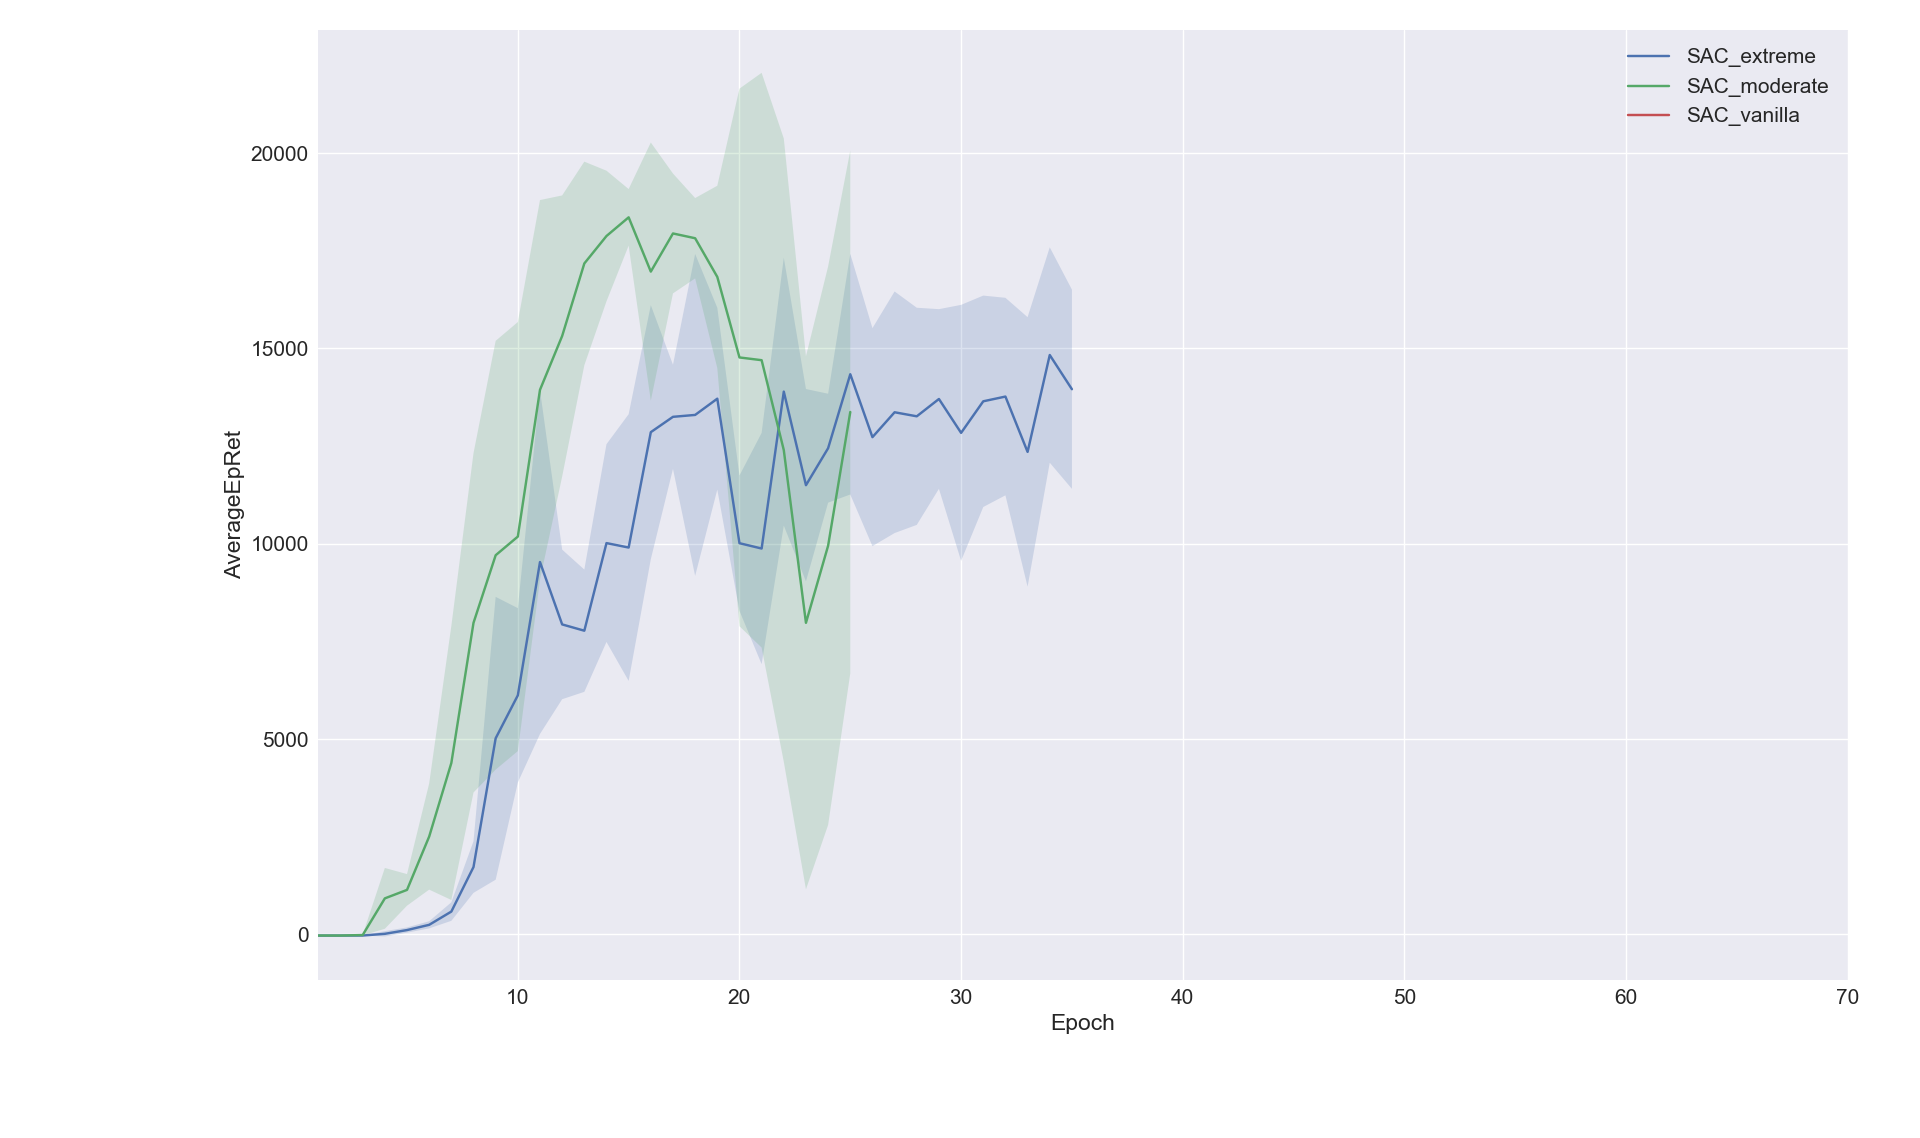
\includegraphics[width = .82\textwidth]{img/return_SAC.png}
%      \end{subfigure}
%     \caption{TD3 and SAC cumulative return for the vanilla training case. Given 
%     that 5 runs were executed, the plot reflects the average and standard deviation 
%     corresponding to the learning process of the 5 agents.}
%     \label{fig:ok_training}
% \end{figure}

\begin{figure}[H]
    \centering
     \begin{subfigure}[b]{\textwidth}
         \centering
             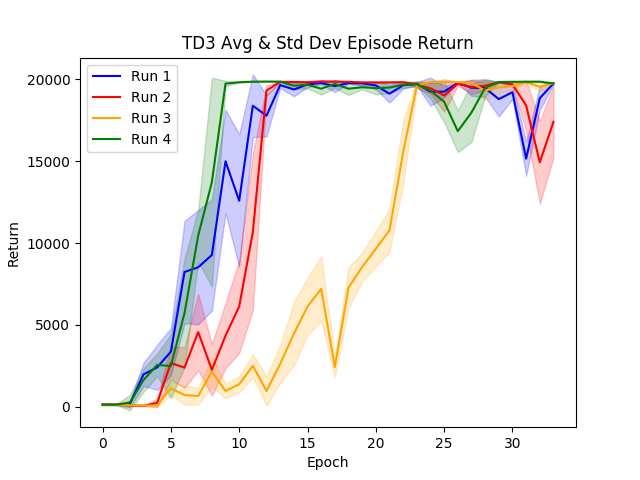
\includegraphics[width = .5\textwidth]{img/TD3_return_vanilla.png}
        \caption{Drone Hovering}
     \end{subfigure}
    % \hfill 
     \begin{subfigure}[b]{\textwidth}
         \centering
             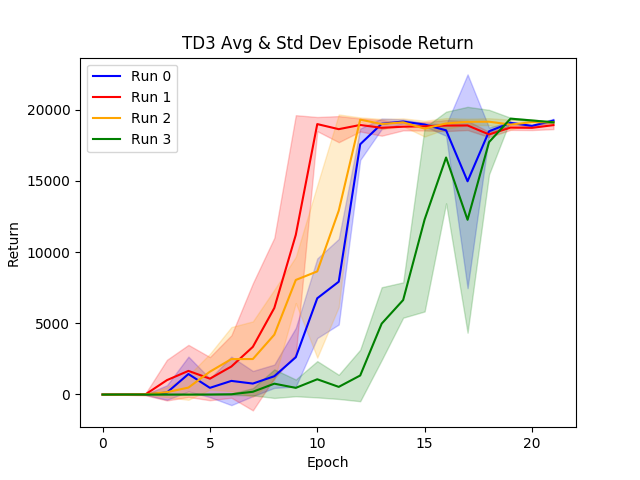
\includegraphics[width = .5\textwidth]{img/TD3_return_moderate.png}
         \caption{Drone Navigation from A to B}
     \end{subfigure}
    %  \hfill
     \begin{subfigure}[b]{\textwidth}
         \centering
             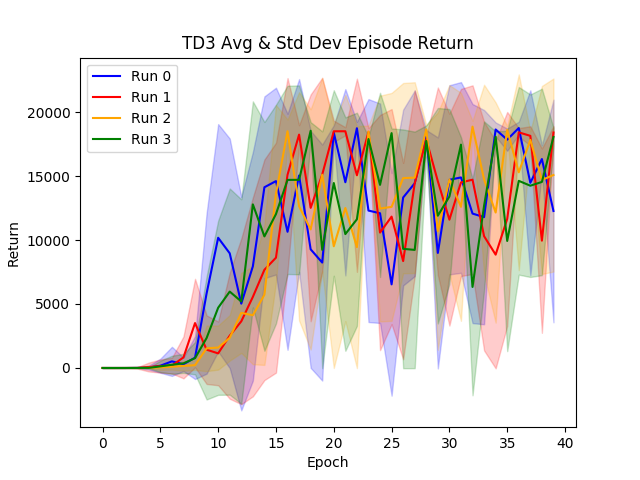
\includegraphics[width = .5\textwidth]{img/TD3_return_extreme.png}
         \caption{Drone Navigation with harder initial conditions}
     \end{subfigure}
    \caption{TD3 Average return per episode. We can see that TD3 performs much better than VPG, PPO, and DDPG, and it achieves much higher returns.}
    \label{fig:td3}
\end{figure}

\begin{figure}[H]
    \centering
     \begin{subfigure}[b]{\textwidth}
         \centering
             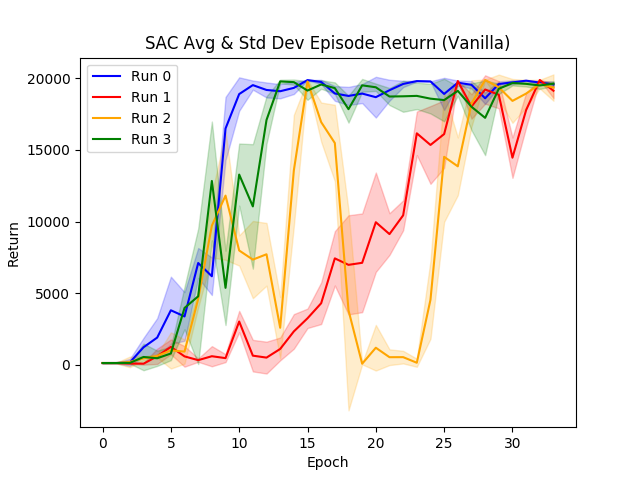
\includegraphics[width = .5\textwidth]{img/SAC_return_vanilla.png}
             \caption{Drone Hovering}
     \end{subfigure}
    \hfill 
     \begin{subfigure}[b]{\textwidth}
         \centering
             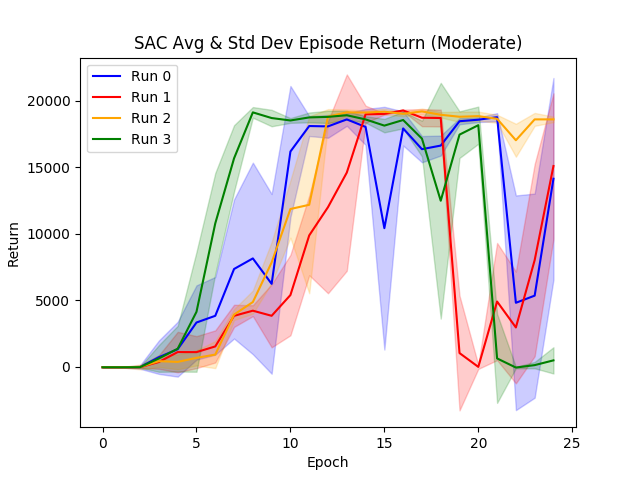
\includegraphics[width = .5\textwidth]{img/SAC_return_moderate.png}
             \caption{Drone Navigation from A to B}
     \end{subfigure}
     \hfill
     \begin{subfigure}[b]{\textwidth}
         \centering
             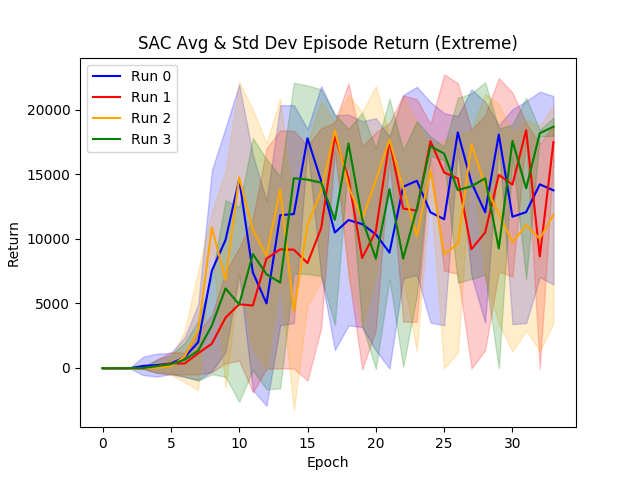
\includegraphics[width = .5\textwidth]{img/SAC_return_extreme.png}
             \caption{Drone Navigation with harder initial conditions}
     \end{subfigure}
    \caption{SAC Average return per episode. SAC does seem to converge to an optimal, but it clearly is not as stable as TD3. This may be due to SAC's entropy regularization.}
    \label{fig:sac}
\end{figure}

\subsection{Testing the agents} % Graph state and action 

The trained agents were tested in a controlled test-bed. That is, selecting a testing scenario 
(vanilla, moderate, extreme) and running the policy the agents learnt in training. 
Table~\ref{tab:testing_conditions} shows the scenarios used. It is possible to appreciate that 
each scenario consists of 4 different tests, were the initial state vector is modified.

\begin{table}[H]
    \centering
    \caption{Testing conditions.}
    \label{tab:testing_conditions}
    \begin{tabular}{l|c c c c}
        \toprule[0.5pt]
    \textbf{Training condition} & Position [m]        & Euler angle [deg]   & Velocity [m/s]        & $\omega$ [rad/s]      \\
    \midrule[1pt]
                                & $[-.6, .8, 3.5]^T$  & $[0, 0, 0]^T$       & $[0, 0, 0]^T$         & $[0, 0, 0]^T$         \\
    Vanilla                     & $[ 0,  0,  3.0]^T$  & $[0, 0, 0]^T$       & $[0, 0, 0]^T$         & $[-.01, .005, .002]^T$\\
                                & $[ 0,  0,  3.0]^T$  & $[5, -2, 0]^T$      & $[0, 0, 0]^T$         & $[0, 0, 0]^T$         \\
                                & $[0, 0, 3.0]^T $    & $[0, 0, 0]^T$       & $[.1, .05, .01]^T$    & $[0, 0, 0]^T$         \\
    \midrule[1pt]
                                & $[-.6, .8, 3.5]^T$  & $[-30, 25, 0]^T$    & $[0, 0, 0]^T$         & $[0, 0, 0]^T$         \\
    Moderate                    & $[.5, -.4, 3.7]^T$  & $[0, 0, 0]^T$       & $[.3, -.24, .1]^T$    & $[0, 0, 0]^T$         \\
                                & $[.7, -.4, 2.5]^T$  & $[0, 0, 0]^T$       & $[0, 0, 0]^T$         & $[.15, -.2, .1]^T$    \\
                                & $[.5, -.4, 2.7]^T$  & $[-20, 30, 0]^T$    & $[0, -.05, .09]^T$    & $[-.05, .15, -.08]^T$ \\
    \midrule[1pt]
                                & $[-.6, .8, 3.5]^T$  & $[-80, 85, 180]^T$  & $[0, 0, 0]^T$         & $[0, 0, 0]^T$         \\
    Extreme                     & $[.5, -.4, 3.7]^T$  & $[0, 0, 0]^T$       & $[1.8, -1.6, -1.4]^T$ & $[0, 0, 0]^T$         \\
                                & $[.7, -.4, 2.5]^T$  & $[0, 0, 0]^T$       & $[0, 0, 0]^T$         & $[1.35, -1.5, 1.1]^T$ \\
                                & $[.5, -.4, 3.0]^T$  & $[60, 85, 0]^T$     & $[1.3, -1.2, -.9]^T$  & $[-.45, .35, .18]^T$  \\
        \bottomrule[2pt]
    \end{tabular}
\end{table}


We generated graphs for some of these test cases, and we walk through them below.

\subsubsection{Example - Moderate Agents}

In the following two figures, we show that the agents we trained to travel from their initial state to a goal state are able to hover in place (Figure~\ref{fig:moderate_vanilla_3}) and also travel from one state to another (Figure~\ref{fig:moderate_moderate_0}). The graphs 
show only 400 steps but that is just a visualization decision we adopted to be able to show the 
transition from initial condition to hover. Longer episodes were studied and the agents 
reach a steady state no matter how long the simulation is.

\begin{figure}[H]
    % \centering
    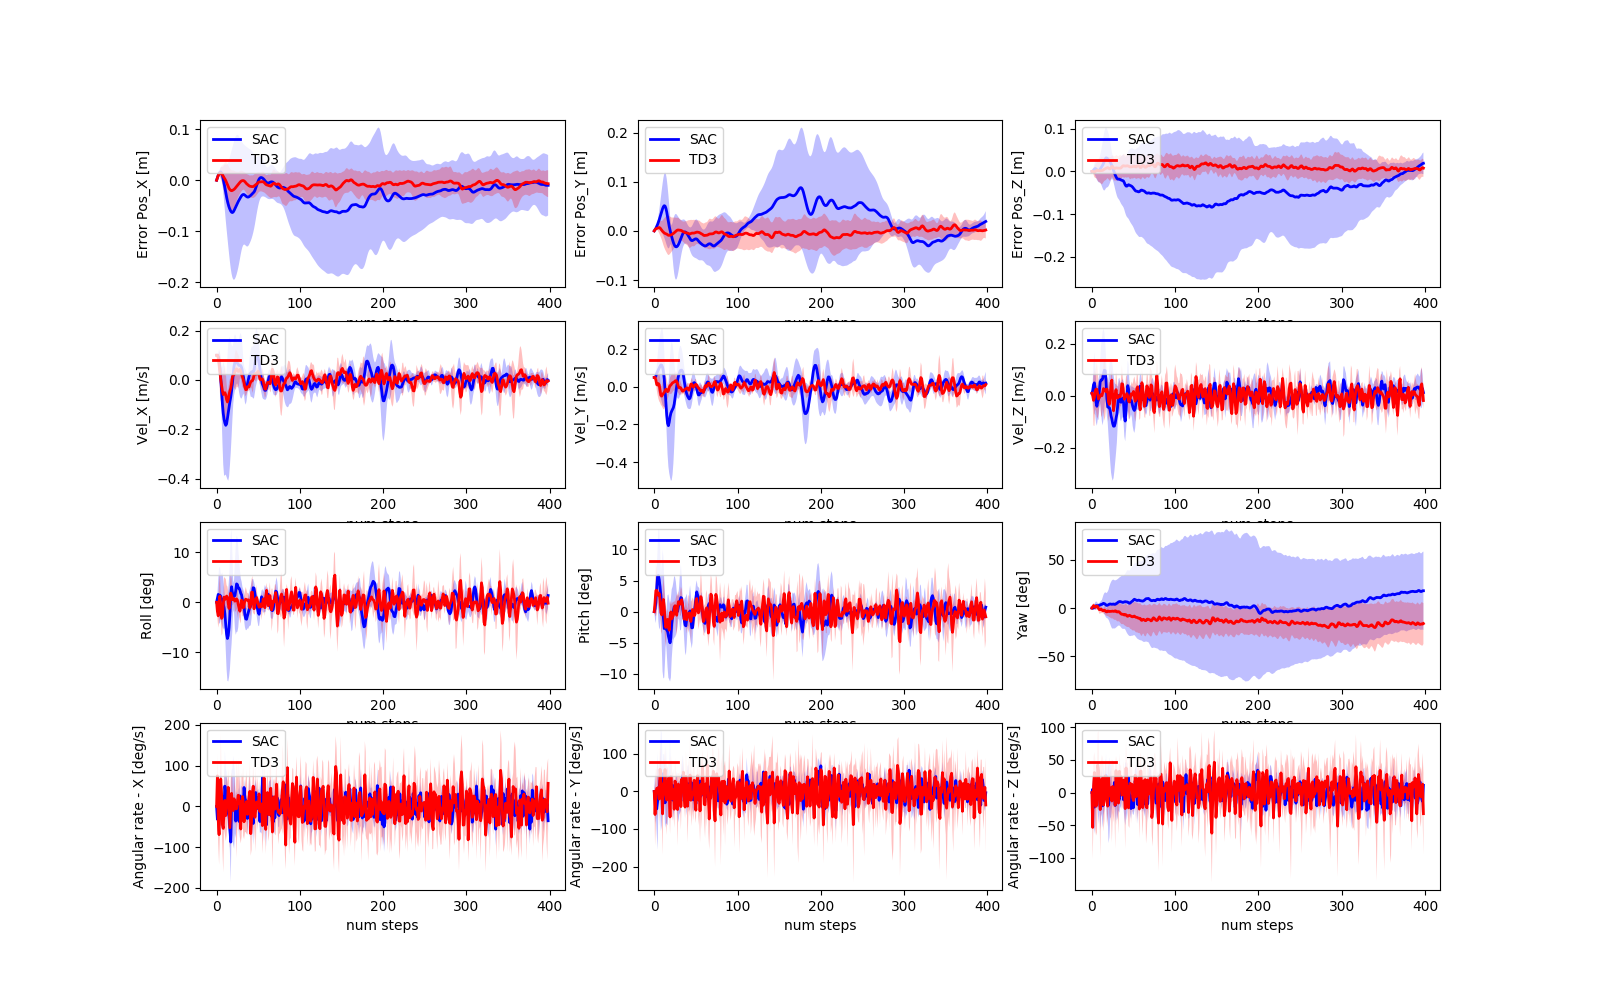
\includegraphics[width = 1\textwidth]{img/2022-05-05_00:00:00_moderate_states_3_vanilla.png}
    \caption{Moderate training and fourth test case of the moderate initialization. Given 
    that 5 runs were executed, the plot reflects the average and standard deviation 
    corresponding to the testing process on the 5 agents.}
    \label{fig:moderate_vanilla_3}
\end{figure}

\begin{figure}[H]
    % \centering
    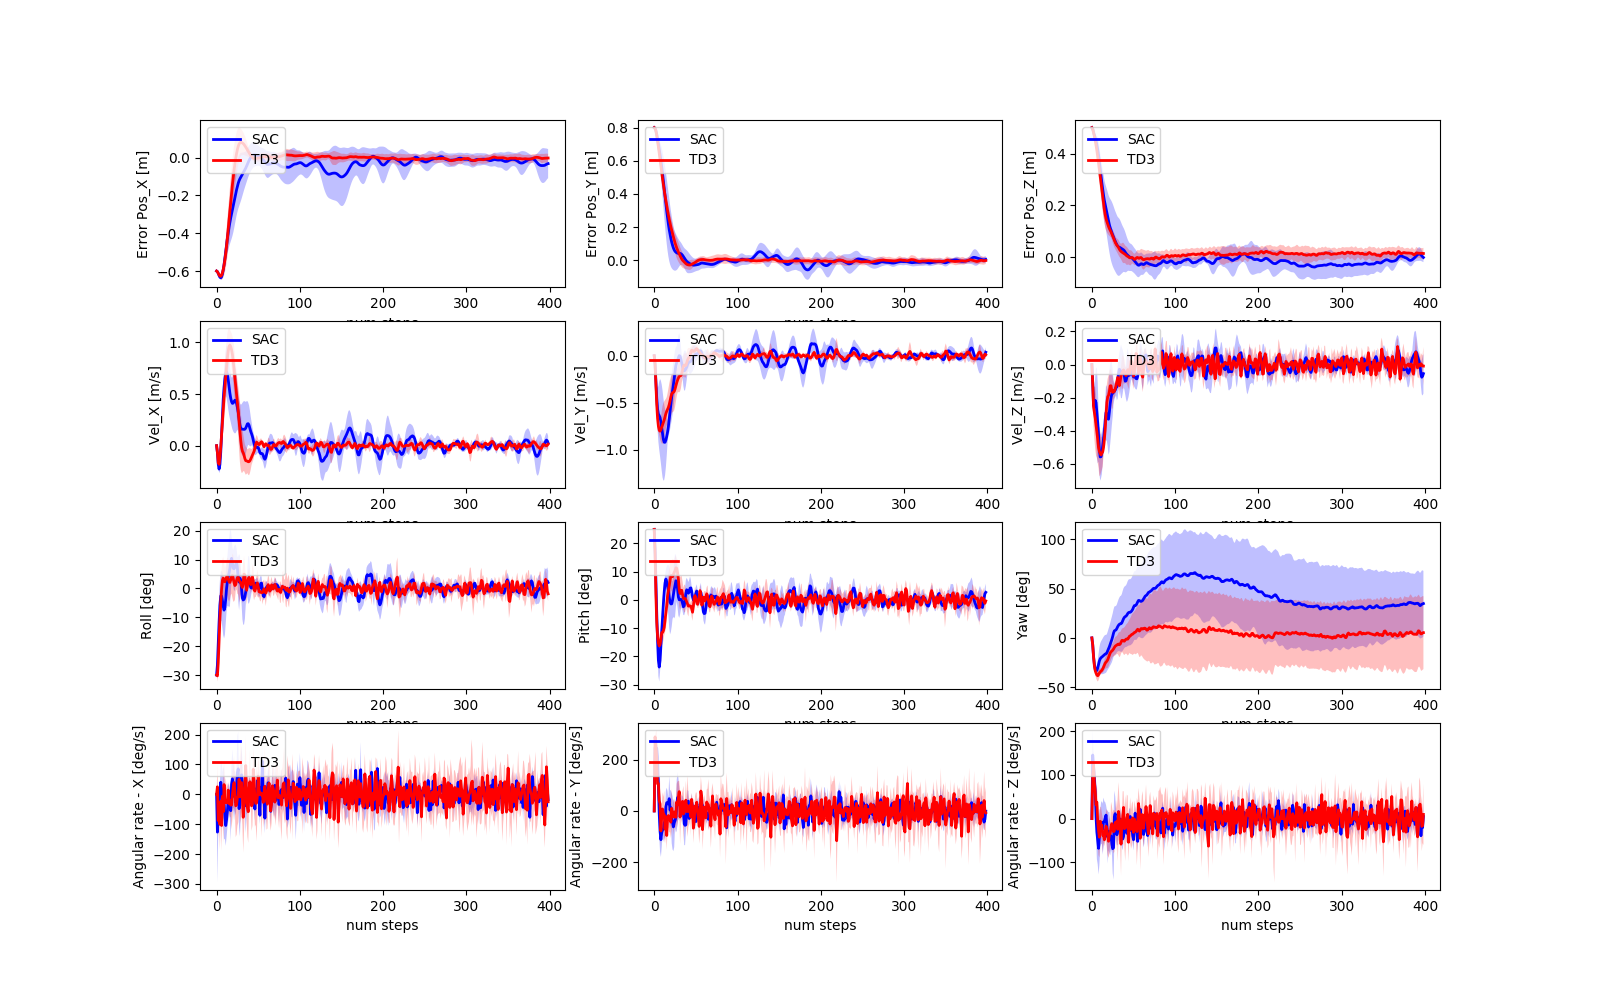
\includegraphics[width = 1\textwidth]{img/2022-05-05_00:00:00_moderate_states_0_moderate.png}
    \caption{Moderate training and first test case of the moderate initialization. Given 
    that 5 runs were executed, the plot reflects the average and standard deviation 
    corresponding to the testing process on the 5 agents.}
    \label{fig:moderate_moderate_0}
\end{figure}

It is interesting to note that in the third test of the moderate scenario (Figure~\ref{fig:moderate_moderate_3} one can appreciate the difference in performance
between TD3 and SAC. Here, at least one of the drones trained with SAC flies out of 
the bounding box represented by an allowed position error and therefore the episode 
ends. This further illustrates that TD3 was more robust when evaluating our trained agents.

\begin{figure}[H]
    % \centering
    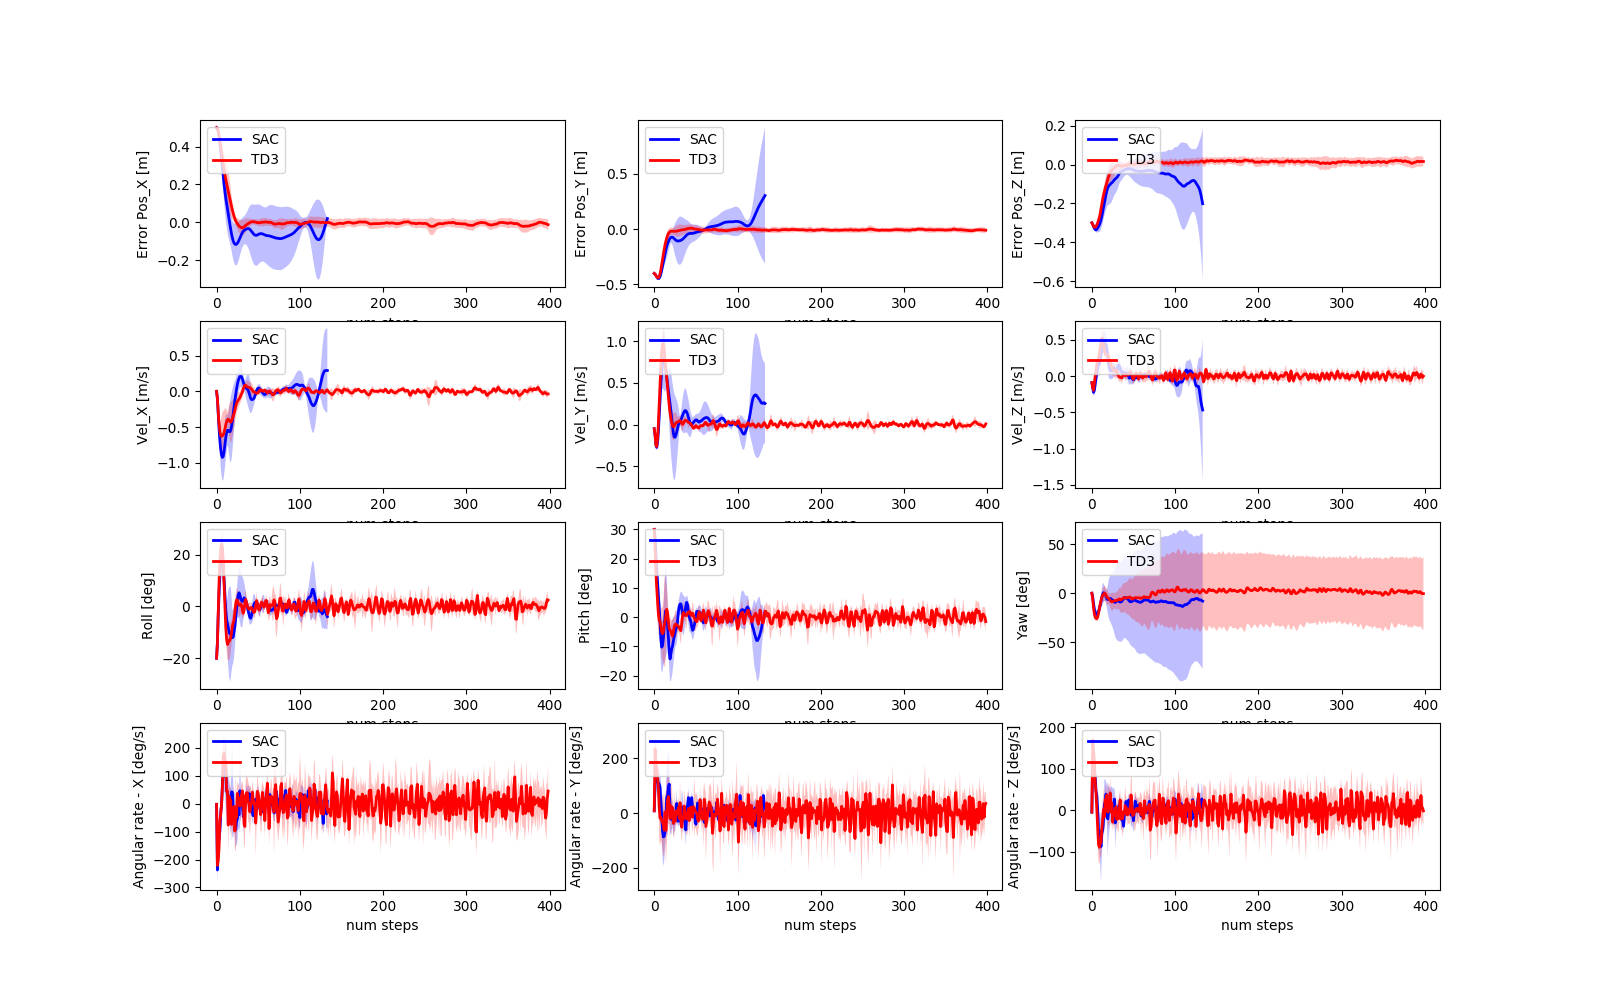
\includegraphics[width = 1\textwidth]{img/2022-05-05_00:00:00_moderate_states_3_moderate.png}
    \caption{Moderate training and fourth test case of the moderate initialization. Given 
    that 5 runs were executed, the plot reflects the average and standard deviation 
    corresponding to the testing process on the 5 agents.}
    \label{fig:moderate_moderate_3}
\end{figure}

\subsubsection{Extreme training}

Handling the extreme case is something that we wanted to test because it would mean that the agent 
is very likely to recover from aggressive maneuvers as we are testing here. But it would 
also mean that acrobatic drones could in fact be implemented through proper training. This 
fact is not minor, since traditional control methods would not be able to handle those cases.
Therefore, our results not only come from a model-free learning process but also beats some 
traditional methods in what they can handle.

Figure~\ref{fig:extreme_extreme_1} indeed shows that the agents were able to learn 
how to recover from very challenging initial conditions and at the same time move 
to a certain location. Once again, we can see that TD3 was more robust than SAC, and its agents had less variation in the policy they learned.

\begin{figure}[H]
    \centering
    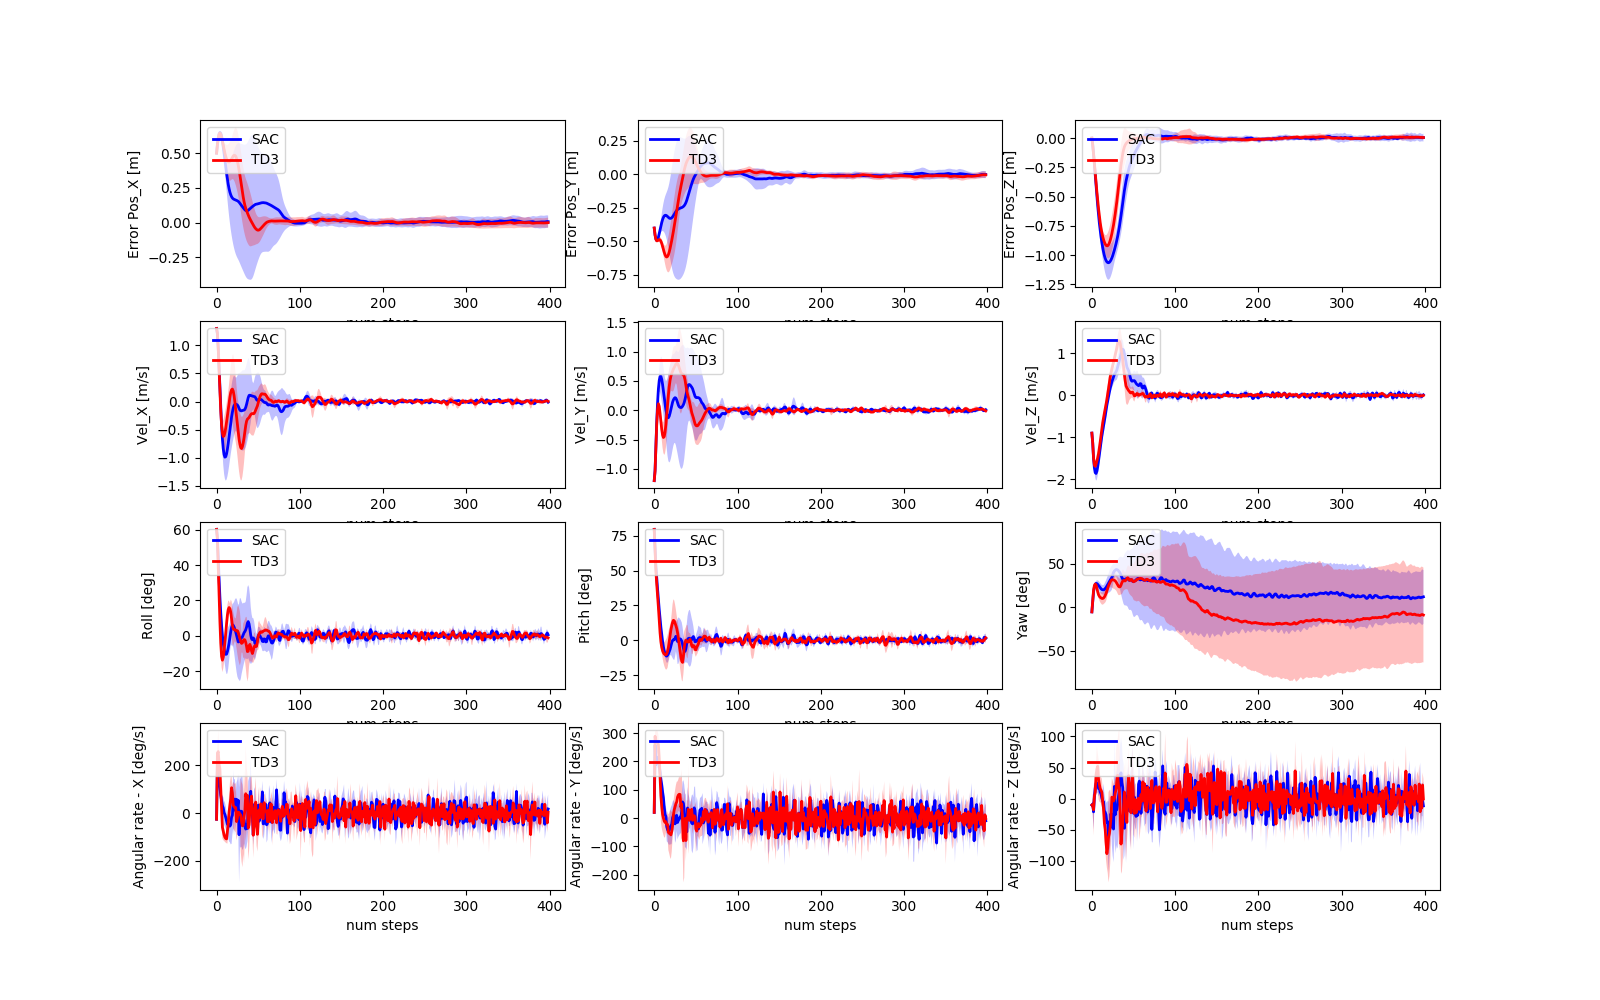
\includegraphics[width = 1\textwidth]{img/2022-05-05_00:00:00_extreme_states_3_extreme.png}
    \caption{Extreme training and fourth test case of the extreme initialization. Given 
    that 5 runs were executed, the plot reflects the average and standard deviation 
    corresponding to the testing process on the 5 agents.}
    \label{fig:extreme_extreme_1}
\end{figure}

\subsection{Following a Trajectory}

After training the drone, we found that the TD3 agent learned the most robust policy. We wanted to see how accurately our trained agent could follow a set of trajectories, especially after we added reward for staying close to the straight line between start and goal. Below, we can see a graph illustrating the top-down view of our drone as it flies along a square trajectory. For 3 out of 4 sides of the square, we can see it follows the trajectory accurately. However, for some reason, it seems the agent never had a chance to learn a better policy for navigating to the left.


\begin{figure}[H]
    \centering
    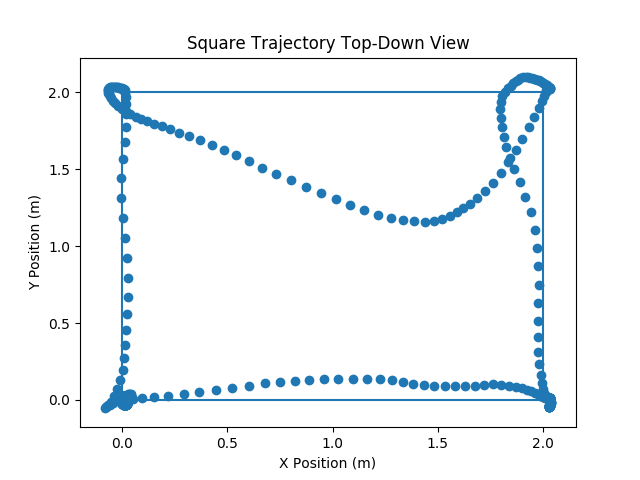
\includegraphics[width = 1\textwidth]{img/square.png}
    \caption{A top-down plot of the drone's position following a 2m square at a fixed height. The drone gets off course on the top edge of the square, but follows the trajectory relatively well for the other edges.}
    \label{fig:square}
\end{figure}

Trying to make a finer trajectory with more intermediate goals, we see that there is a consistent erroneous behavior. The drone is always veering to the left before arriving at its goal. Adding different incentives to our reward function somewhat helped follow the lines better, but it still is not very precise.

\begin{figure}[H]
    \centering
    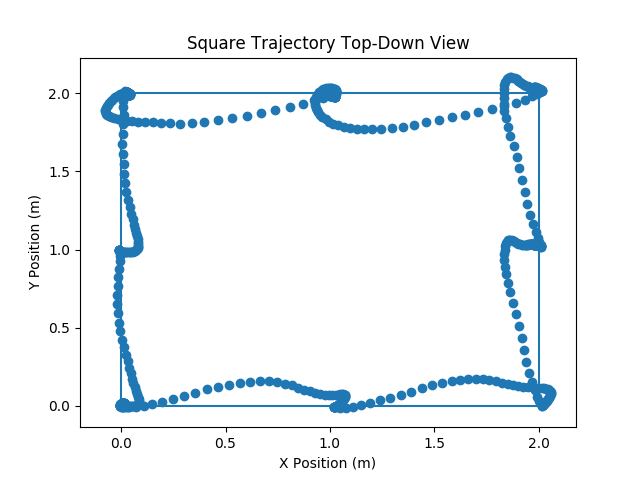
\includegraphics[width = 1\textwidth]{img/finer_square.png}
    \caption{A top-down plot of the drone's position following a 2m square trajectory at a fixed height, with target points more frequently placed along the trajectory. There is a consistent swerve to the left before reaching each target point.}
    \label{fig:finer_square}
\end{figure}